\chapter{基于通道相关性的彩色图像可逆隐藏}
\label{c:proposed}
在本章中将首先对本论文提出的二阶预测算法和嵌入算法进行介绍,然后将给出新的像素排
序算法,在第三节会给出完整的嵌入流程,最后是对实验结果的分析总结。


\section{预测嵌入}
尽管一个像素的三个通道之间存在一定的联系,但是它们并没有明显的通道相关性。下图是
lena图像红-绿通道像素差的直方图同预测误差直方图的对
\begin{figure}[!h]
\centering 
\subfigure[lena图像R-B直方图]{
  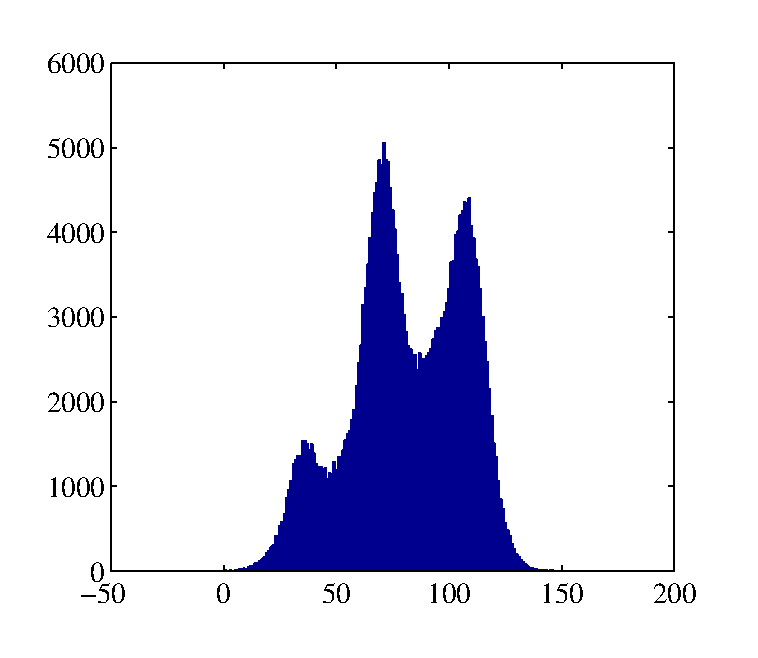
\includegraphics[width=0.4\textwidth]{figures/lena_r_g.eps}
  \label{fig:lena_rg_hist}}
\subfigure[lena图像预测误差直方图]{
  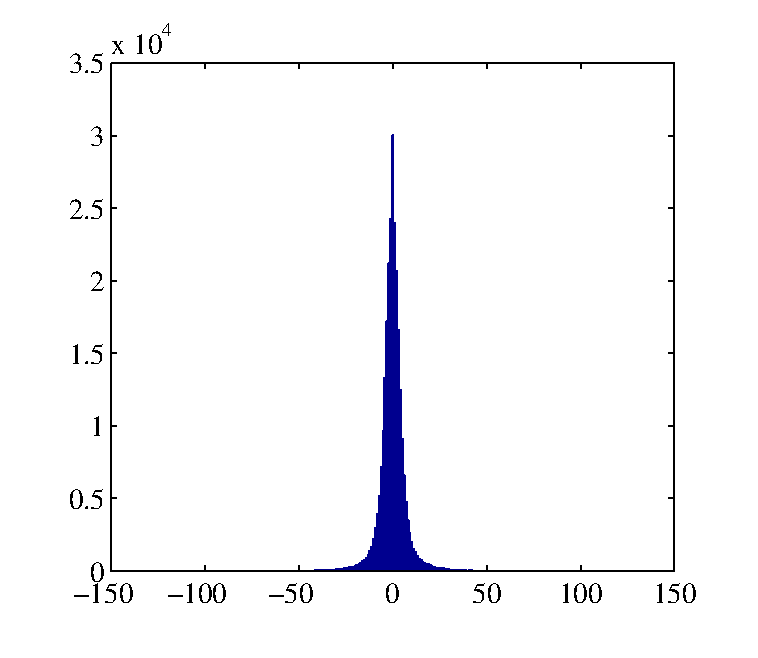
\includegraphics[width=0.4\textwidth]{figures/lena_diffhist.eps}
  \label{fig:lena_diffhist2}}
\caption{lena图像灰度直方图同预测误差直方图的比较}
\label{fig:lena_rg_pe_compare}
\end{figure}
比。我们可以看到直接的像素差的方差很大,且没有明显的规律可寻。因此,现在常用的
算法都针对预测误差进行平移扩展。
\par
然而,一般的预测算法在图像的纹理复杂区域的预测效果却并不理想。在这种情况下,由于
邻域像素同被预测像素的巨大差异,预测值通常与正确值有着很大的差异。另一方面,由于
彩色图像存在三个通道,通道间的高度的相关性为在图像纹理复杂区域的预测提供了帮助,
当对一个通道内的像素进行预测时,我们可以利用另一个通道的信息来辅助当前通道进行更
准确的预测。图\ref{fig:lena_rgb_pe_compare}分别是Lena图像利用一般的预测算法分别
对RGB三个通道进行预测之后的预测误差图。
\begin{figure}[!h]
\centering 
\subfigure[R通道预测误差图]{
  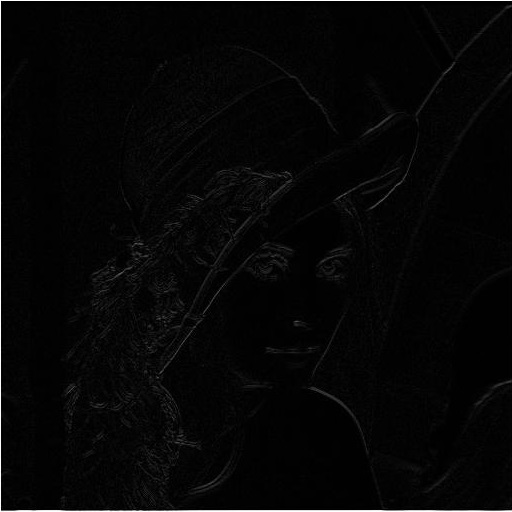
\includegraphics[width=0.3\textwidth]{figures/lena_pe_r.jpg}
  \label{fig:lena_rpe_hist}}
\subfigure[G通道预测误差图]{
  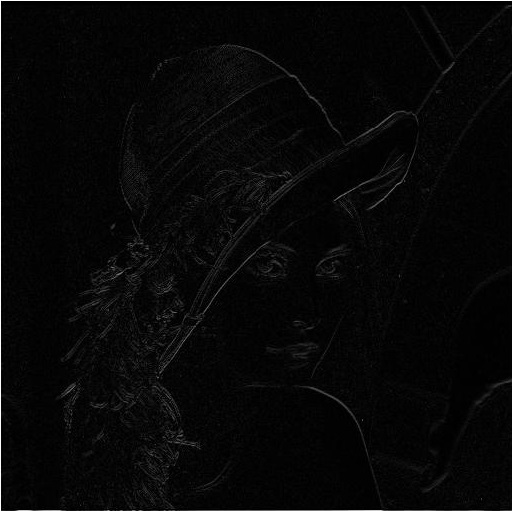
\includegraphics[width=0.3\textwidth]{figures/lena_pe_g.jpg}
  \label{fig:lena_gpe_hist}}
\subfigure[B通道预测误差图]{
  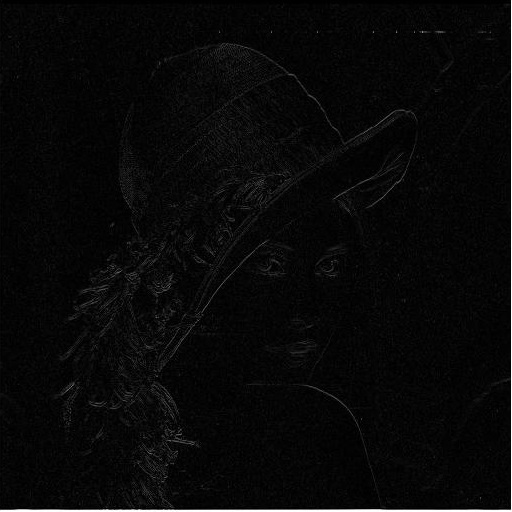
\includegraphics[width=0.3\textwidth]{figures/lena_pe_b.jpg}
  \label{fig:lena_bpe_hist}}
\caption{lena图像三个通道预测误差图像对比}
\label{fig:lena_rgb_pe_compare}
\end{figure}
从图中我们可以看到,如果一个像素在当前通道内可以被准确预测,那么在另外两个通道
也基本可以被准确预测;对于纹理复杂区域,在三个通道基本都不能做出很准确的预测,
然而三个通道的预测误差却很相似。因此,如果我们在一个通道内对一个像素求出了一个
预测误差$e$,那么我们可以推测在另一个通道内的预测误差应该同$e$是很接近的。
\par
这样,在本文提出的可逆隐藏算法中,数据同样是分别嵌入到每一个通道中。但是在对当
前的通道进行预测的过程中,我们会选取另外一个参考通道同样进行一次预测,得到一个
参考预测误差对当前通道的预测误差进行二次预测。在本文的算法中,依然使用Sachev提
出的棋盘格格式的两轮预测的算法。对于一个像素$I$,设当前通道内的像素表示为$I_c$,
参考通道内的像素表示为$I_r$。图\ref{fig:pixel_neighbour2}表示一个像素的8个邻域
像素。
\begin{figure}
  \centering
  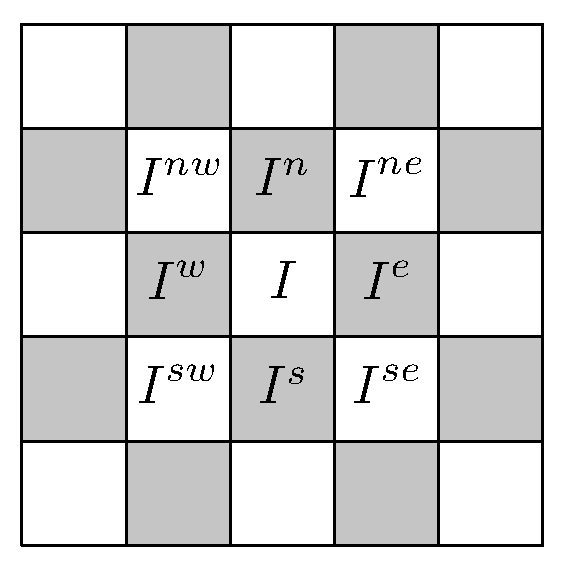
\includegraphics[width=0.3\textwidth]{figures/pixel_neighbourhood.eps}
  \caption{像素$I$的邻域像素}
  \label{fig:pixel_neighbour2}
\end{figure}
\par
首先对当前通道内的像素$I_c$求其预测值$\hat{I}_c$和通道内一阶预测误差$e_{1c}$:
\begin{eqnarray}
  & \displaystyle \hat{I}_c=
    \left\lfloor \sum_{k=1}^8\lambda_c^kI_c^k+0.5 \right\rfloor & \\
  & e_{1c}=I_c-\hat{I}_c &
  \label{eq:current_predict}
\end{eqnarray}
\par
其中$\lambda_c^k$为预测算法中对邻域像素的权重,可以如文献
\cite{sachnev2009reversible}中,选取上下左右权重为$1/4$,或者如文献
\cite{luo2010reversible}中,基于插值自适应的选取系数,或者如文献
\cite{li2013reversible}中的权重选取算法;$I_c^k$为像素的8个邻域点。显然,在纹理
平滑区域,$e_{1c}$的值应该较小,而在纹理平滑区域,$e_{1c}$的值较大。这样,对参
考通道的像素求其预测值$I_r$和通道内一阶预测误差$e_{1r}$:
\begin{eqnarray}
  & \displaystyle \hat{I}_r=
    \left\lfloor \sum_{k=1}^8\lambda_r^kI_r^k+0.5 \right\rfloor & \\
  & e_{1r}=I_r-\hat{I}_r &
  \label{eq:reference_predict}
\end{eqnarray}
\par
此时我们得到了当前通道预测误差$e_{1c}$和参考通道预测误差$e_{1c}$,我们求当前像素
$I_c$的二阶预测误差$e_2$:
\begin{equation}
  e_2=e_{1c}-e_{1r}
  \label{eq:second_predict}
\end{equation}
\par
我们知道,在平滑区域预测算法都可以预测的很准确。这样$e_{1c}$和$e_{1r}$都接近于0,
二阶误差$e_2$同样接近于0;而对于纹理复杂区域,$e_{1c}$和$e_{1r}$都相对较大,但
是由于前面所述的通道间相关性,二阶误差$e_2$同样会较小。
\par
预测算法的效果的好坏通常由预测误差直方图的陡峭程度来衡量,数值化之后就是预测误差
的熵值。熵越小,预测结果就越准确。我们对UCID数据库\cite{schaefer2003ucid}中超
1300副图像都进行了考察。对每一幅图像,我们计算了论文预测算法的熵值和另外几种算法
的熵值。从图\ref{fig:entropy_compare}中可以看出,几乎对所有的图像我们提出的预测
算法的熵值都比以往算法的熵值要小。这在统计上证明了提出的预测算法可以比以往算法
获得更准确的预测误差。
\par
接下来,参考传统的预测误差扩展算法,定义两个阈值$T_r$和$T_l$,将预测误差直方图
分为一个扩展区域和两个平移区域。对不同区域的二阶预测误差$e_2$进行扩展或者平移,
即:
\begin{equation}
  e_2^{'}=\left\{ \begin{array}{ll}
    2e_2+b & if~~e_2 \in [T_r,T_l)\\
    e_2+T_r & if~~e_2 \ge T_r\\
    e_2+T_l & if~~e_2<T_l
  \end{array} \right.
  \label{eq:second_pe_embedding}
\end{equation}
\begin{figure}
  \centering
  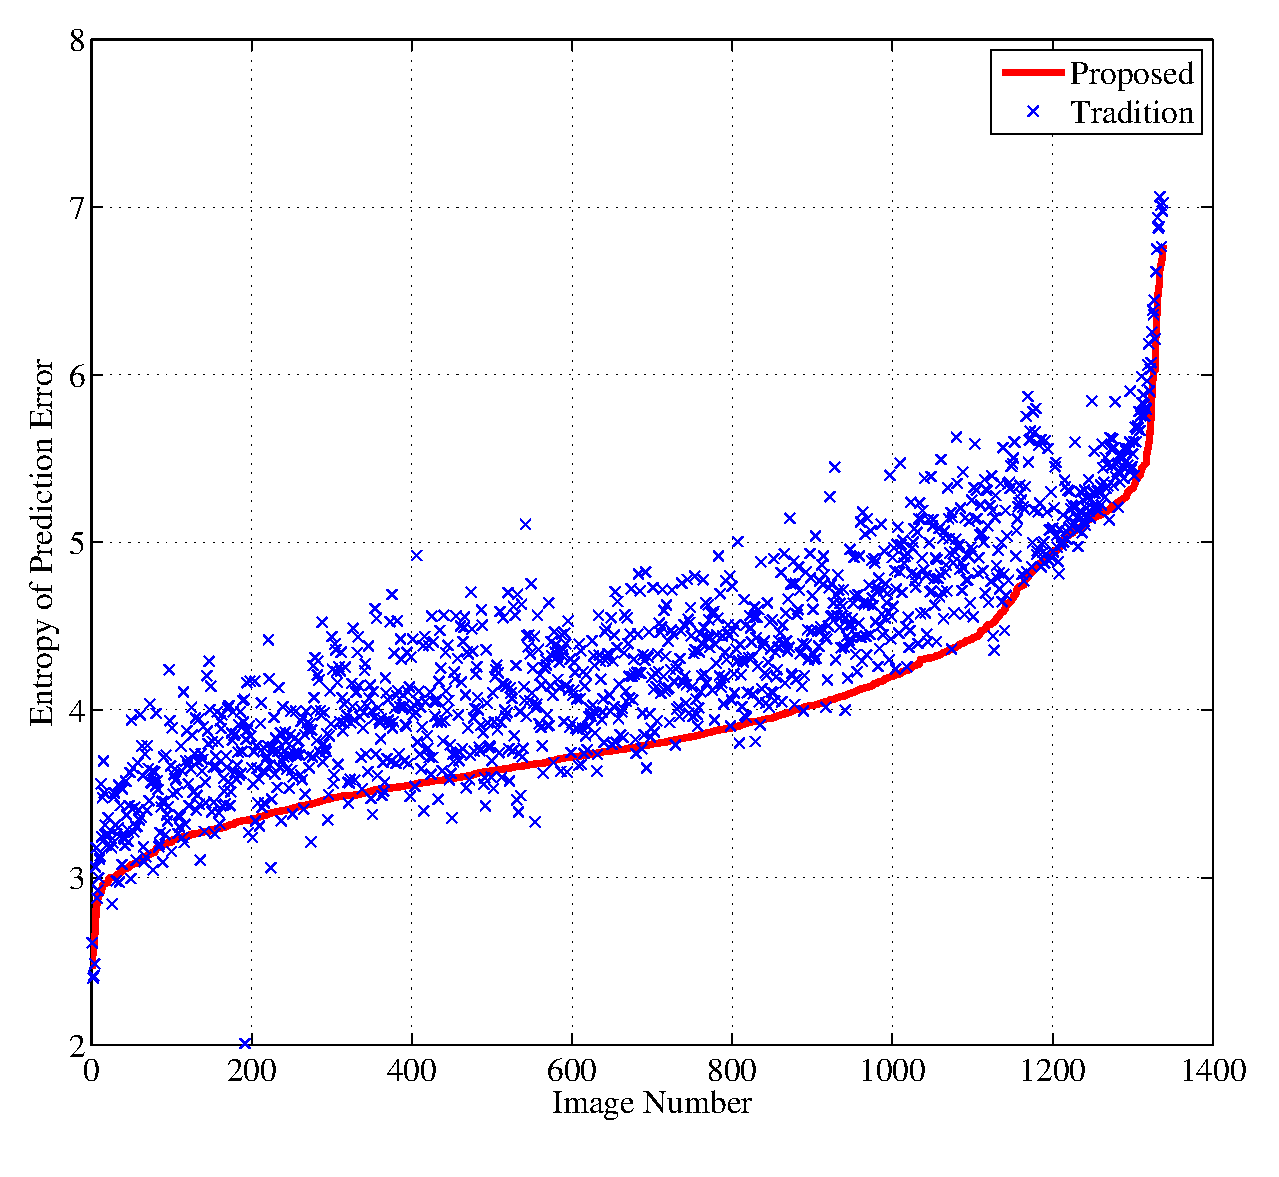
\includegraphics[width=0.65\textwidth]{figures/entropy_compare.eps}
  \caption{预测误差直方图熵比较}
  \label{fig:entropy_compare}
\end{figure}
其中$b\in\{0,1\}$为1比特要嵌入的信息。将修改后的二阶误差加到使用参考通道预测的
一阶预测误差上得到:
\begin{equation}
  e_{1c}^{'}=e_{1r}+e_2^{'}
  \label{eq:cur_first_pe_embedding}
\end{equation}
最后将修改后的一阶误差加到当前通道的预测值上得到修改后的像素值:
\begin{equation}
  I_c^{'}=\hat{I}_c+e_{1c}^{'}
  \label{eq:marked_pixel}
\end{equation}
\par
在消息提取端,首先求当前通道的预测值$\hat{I}_c$和参考通道的预测值$\hat{I}_r$,
求得修改后的当前通道的误差$e_{1c}^{'}$和参考误差$e_{1r}$,从而计算得出修改后的
二阶误差$e_2^{'}$。显然消息比特$b$为二阶误差的最低有效位,即:
\begin{equation}
  \begin{array}{ll}
    \displaystyle b=e_2^{'}-2\left\lfloor\frac{e_2^{'}}{2}\right\rfloor & 
    if~~e_2^{'}\in[2T_l,2T_r)
  \end{array}
  \label{eq:data_extraction}
\end{equation}
\par
为了恢复原始像素,首先恢复原始二阶预测误差:
\begin{equation}
  e_2=\left\{ \begin{array}{ll}
    \displaystyle \left\lfloor\frac{e_2^{'}}{2}\right\rfloor &
    if~~e_2^{'} \in [2T_r,2T_l)\\
    e_2^{'}-T_r & if~~e_2^{'} \ge 2T_r\\
    e_2^{'}-T_l & if~~e_2^{'}<2T_l
  \end{array} \right.
  \label{eq:second_pe_restoration}
\end{equation}
从而根据\ref{eq:second_predict}和\ref{eq:current_predict}的逆过程恢复当前通道
的一阶预测误差和原始像素。




\section{像素排序与位置地图}
嵌入算法的效果可以通过进一步的排序得到提升。根据像素的纹理复杂度将像素进行排序,
使纹理平滑的像素,即预测误差更小的像素尽可能多的被修改。根据嵌入公式,我们知道,
被嵌入的像素的失真为其预测误差,被移动的像素失真为阈值$T_r$或者$T_l$。由此可以
知道,当修改的像素大多数时候是小误差的像素时,图像失真就会较小。在本节中,将给
出对像素排序和位置地图的细节和数学推导。
\par
如前文所述,理想化的图像预测误差是服从标准拉普拉斯分布的。为了细致的研究预测误
差的分布特征,以在排序中对其加以利用,我们将独立的对每一个像素点的预测误差分布
进行研究。以某个像素点为例,其邻域像素如图\ref{fig:pixel_neighbour2}所示。
\par
首先对当前像素$I$,取其$3\times3$邻域的上下左右四个邻域像素,求得四个差值:
\begin{eqnarray}                           
  & d_1=I^w-I^n & \\
  & d_2=I^n-I^e & \\
  & d_3=I^e-I^s & \\
  & d_4=I^s-I^w &
\end{eqnarray}
设预测误差$e_1$服从参数为$(\mu_1,\lambda_1)$的拉普拉斯分布,令:
\begin{equation}
  \mu_1^1=\frac{1}{2}(d_1+d_3), \mu_1^2=\frac{1}{2}(d_2+d_4)
\end{equation}
取$\mu_1^1$,$\mu_1^2$中较小的一个作为该预测误差分布的期望$\mu_1$再令:
\begin{equation}
  \lambda_1=\sqrt{\frac{1}{4\times2}\sum_{k=1}^{4}(d_k-\mu_1)^2}
\end{equation}
作为该点拉普拉斯分布的参数$\lambda_1$,(标准拉普拉斯分布中方差为$2\lambda_1^2$),
我们就可以得到该待嵌入像素点的一个分布的估计:
\begin{equation}
  f(x)=\frac{1}{2\lambda_1}e^{-\frac{|x-\mu_1|}{\lambda_1}}
  \label{eq:laplace_distr}
\end{equation}
其概率密度函数图像如图\ref{fig:laplace_distr}:
\begin{figure}[!h]
\centering 
\subfigure[概率分布情况1]{
  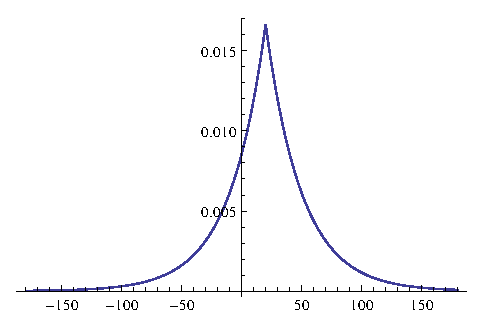
\includegraphics[width=0.3\textwidth]{figures/laplace1.eps}
  \label{fig:laplace1}}
\subfigure[概率分布情况2]{
  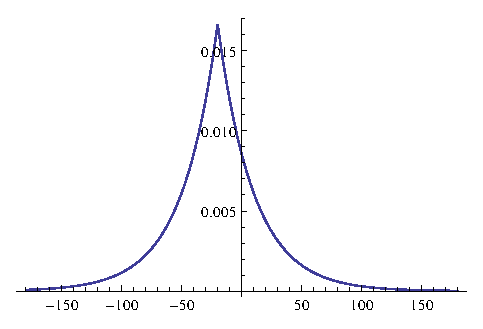
\includegraphics[width=0.3\textwidth]{figures/laplace2.eps}
  \label{fig:laplace2}}
\subfigure[$g(x)$概率分布图]{
  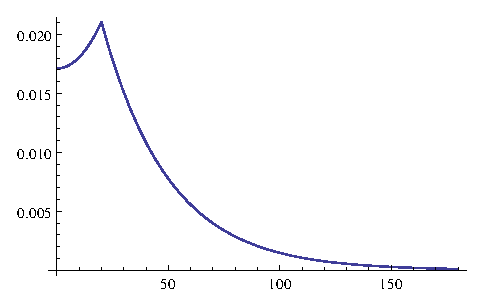
\includegraphics[width=0.3\textwidth]{figures/laplace3.eps}
  \label{fig:laplace_distr_new}}
\caption{$f(x)$和$g(x)$概率分布图}
\label{fig:laplace_distr}
\end{figure}
\par
由图像可以看出,$\mu$到$y$轴的距离大小可以用来反映预测误差的准确程度,$\mu$到$y$
轴越近,则预测误差越接近0,因而预测的越准确。
\par
由于使用了$\mu$到$y$轴的距离来衡量预测误差的准确程度,因此可以将拉普拉斯分布位于
$x$轴负半边的图像取绝对值,翻转到$x$轴正半边,得到一个新的概率密度图像如图\ref{fig:laplace_distr_new}:
\par
设其概率密度函数为$g(x)$,其期望值是一个与$\mu$的绝对值(即$\mu$到0轴的距离)正
相关的数(具体计算结果将在下文给出),因此我们可以利用$g(x)$的期望值$E[g(x)]$作
为当前像素预测误差准确性的度量,用其对像素进行排序,这是本文排序算法的核心。
\par
设当前待嵌入像素的预测误差的分布为公式\ref{eq:laplace_distr},不妨假设此时$\mu>0$
(小于0时对 取绝对值即可),则此时$g(x)$是一个分段函数:
\begin{equation}
  g(x)=\left\{ \begin{array}{ll}
    \frac{1}{2\lambda}e^{-\frac{\mu-x}{\lambda}}+\frac{1}{2\lambda}e^{-\frac{\mu+x}{\lambda}} &
    if~~0\le x\le\mu\\
    \frac{1}{2\lambda}e^{-\frac{x-\mu}{\lambda}}+\frac{1}{2\lambda}e^{-\frac{\mu+x}{\lambda}} &
    if~~x\ge\mu\\
  \end{array} \right.
  \label{eq:second_pe_embedding}
\end{equation}
其期望为:
\begin{equation}
  E[g(x)]=\int_0^{\infty}xg(x)dx=\lambda e^{-\frac{\mu}{\lambda}}+\mu
\end{equation}
则对当前像素预测误差准确程度的度量为$\lambda e^{-\mu/\lambda}+\mu$。其中$\mu$和
$\lambda$由前文可知。可以很容易的看出,$E$是关于$\mu$和$\lambda$的递增函数,显然
$\mu$和$\lambda$越小,相应地$E$也越小,从而表示预测越精准。因此$E$能很好地反映出
当前像素邻域的纹理复杂性和预测精准度。
\par
在本算法中,由于使用了参考通道的预测误差去预测当前通道的预测误差,因此仅仅使用$E$
来进行排序是不够的。我们在算法中使用
\begin{equation}
  E^{'}=|E_c-E_t|
  \label{eq:sorting_param}
\end{equation}
的方式,表示当前像素两个通道的纹理复杂度的差,差值越小,则表示两个通道在这个像
素点处的结构越相似,因此二阶预测误差也更准。
\par
然而,即使是完美的排序算法也无法避免像素的上溢和下溢问题,因此需要引入位置地图。
我们使用的位置地图构建算法同文献\cite{li2013reversible}的基本相同。当当前像素不
能通过公式\ref{eq:second_pe_embedding}被修改两次时,将在位置地图上记录该像素。
如果像素可以被修改一次,则在位置地图中表示为0;如果像素不能被修改,则在位置地图
中表示为1。然而,由于在预测过程中,使用的邻域像素有可能是载密像素,那么要记录在
位置地图中的像素只有在嵌入的过程中才能确定。即位置地图的构建要在消息嵌入的过程
中同步进行。而如果位置地图和一些辅助信息仍然按照消息的嵌入方式进行嵌入,则有可
能造成新的像素发生上溢或下溢,从而可能要构造另一个位置地图,这样嵌入过程有可能
一直进行。为了解决这个问题,我们将位置地图等信息嵌入到那些值用上、下、左、右四
个邻域进行预测的像素中。这样,嵌入位置地图的那些像素可以提前判断是否会发生上下
溢,从而避免了位置地图的多次构建。



\section{完整流程}
\begin{itemize}
  \setlength{\parindent}{2em}
  \vspace{-2mm}
  \item \textbf{嵌入过程}
    \vspace{-2mm}
    \par
    在本节,基于我们提出的预测算法和排序算法,我们将给出详细的嵌入算法流程。同文
    献\cite{li2013reversible}相同,参考图\ref{fig:three_channel_embedding},我们
    首先以绿色通道为参考通道,将消息嵌入到红色和绿色通道。当嵌入到绿色通道时,以
    已嵌入的红色通道为参考通道。同时,在一个通道中,所有的像素被分为两个集合,以
    灰色和白色像素表示。消息将分为两个阶段分别嵌入到两个集合中,在第一个阶段,将
    消息嵌入到白色的像素中,步骤如下:
    \vspace{2mm}
    \begin{algorithm}[!h]
      \floatname{algorithm}{算法}
      \renewcommand{\algorithmicrequire}{\textbf{输入:}}
      \renewcommand\algorithmicensure {\textbf{输出:}}
      \caption{嵌入算法步骤}
      \label{alg:embedding_step} 
      \begin{algorithmic}[1]
        \REQUIRE ~~\\ %算法的输入参数:Input
        当前通道像素序列,参考通道像素序列,嵌入容量,嵌入消息
        \ENSURE ~~\\ %算法的输出:Output
        载密像素序列
        \vspace{2mm}
        \STATE 设当前阶段待嵌入像素为$\boldsymbol{I}=\{I_1,\dots,I_n\}$,对每
        个像素$I_i$,按照公式\ref{eq:sorting_param}计算其排序权重值$\boldsymbol{V}
        =\{V_1,\dots,V_n\}$,依照$\boldsymbol{V}$的升序,对$\boldsymbol{I}$进行
        排序,得到排序后的像素$\boldsymbol{\tilde{I}}=\{\tilde{I}_1,\dots,
        \tilde{I}_n\}$。
        \STATE 设定阈值初值$T_l$和$T_r$。
        \STATE 将消息嵌入到排序后的像素$\boldsymbol{\tilde{I}}$。对每一个像素
        $\tilde{I}_i (i=1,2,\dots)$,首先根据
        公式\ref{eq:current_predict}--\ref{eq:second_predict}计
        算其预测值和预测误差。根据公式\ref{eq:second_pe_embedding}将消息嵌入到
        像素$\tilde{I}_i$中,得到嵌入消息的像素$\tilde{I}_i^{'}$。然后构建位置地
        图$LM$。如果$\tilde{I}_i^{'}\notin [0,255]$,则$LM(j)=1$,$j=j+1$,将
        $\tilde{I}_i^{'}$改回$\tilde{I}_i$;如果$\tilde{I}_i^{'}\in [0,255]$,但
        是再次嵌入消息后结果不属于$[0,255]$,则$LM(j)=0$,$j=j+1$。
        \STATE 当消息嵌入完成后,记录最后一个嵌入的像素位置为$e$。则
        对$\tilde{I}_i (i=e+1, e+2,\dots, n)$,按照嵌入算法检测所有可嵌入
        的像素的个数,同时记录相应地位置地图。如果可嵌入的像素个数不足以嵌入压缩
        后的$LM$和另外40比特,则将$T_l$减小1(或者将$T_r$增加1),重新开始步骤4。
        否则将$LM$进行可逆压缩,记录压缩后的长度为$l$。
        \STATE 记录当前前40个像素的最低有效位(LSB)为$S_{LSB}$,然后将它们替换为
        $T_r$(8比特),$T_l$(8比特),$l$(8比特)和$e$(16比特)的二进制表示。
        最后将$S_{LSB}$和压缩后的$LM$按照公式\ref{eq:second_pe_embedding}嵌入到
        $e$位置之后的像素中。
      \end{algorithmic}
    \end{algorithm}
    \vspace{-6mm}
    \par
    第二阶段同第一阶段基本相同,只是将待嵌入的像素换成被标记成灰色的像素。
  \vspace{-3.5mm}
  \item \textbf{提取过程}
    \vspace{-2mm}
    \par
    同嵌入过程相反,我们依次从绿色、蓝色、红色通道提取消息,一个通道内的消息提
    取过程也于嵌入过程相反。对每个通道,首先对灰色像素进行提取,提取过程主要分
    为四步。
    \begin{algorithm}[!h]
      \floatname{algorithm}{算法}
      \renewcommand{\algorithmicrequire}{\textbf{输入:}}
      \renewcommand\algorithmicensure {\textbf{输出:}}
      \caption{提取算法步骤}
      \label{alg:embedding_step} 
      \begin{algorithmic}[1]
        \REQUIRE ~~\\ %算法的输入参数:Input
        当前通道载密像素序列,参考通道像素序列
        \ENSURE ~~\\ %算法的输出:Output
        当前通道原始像素,消息
        \vspace{2mm}
        \STATE 找到所有要提取的像素$\boldsymbol{I^{'}}=\{I_1^{'},\dots,I_n^{'}\}$,
        对每个像素进行平滑度打分,得到$\boldsymbol{V}=\{V_1,\dots,V_n\}$,依照
        $\boldsymbol{V}$的升序对载密像素进行排序得到$\boldsymbol{\tilde{I}^{'}}=
        \{\tilde{I}_1^{'},\dots,\tilde{I}_n^{'}\}$
        \STATE 从前40个载密像素提取LSB位,分别恢复$T_r$,$T_l$,$l$和$e$。
        \STATE 按照相反的顺序,从$\{\tilde{I}_{e+l+40}^{'},\dots,\tilde{I}_e^{'}\}$
        的LSB位提取$S_{LSB}$和压缩的$LM$,同时恢复原始的$\{I_{e+l+40},\dots,
        I_{e+1}\}$,对$LM$解压缩,得到原始的位置地图$LM$。
        \STATE 替换前40个载密像素的LSB位为$S_{LSB}$,恢复前40个像素。通过公式%
        \ref{eq:data_extraction}和\ref{eq:second_pe_restoration}提取像素中嵌入
        的消息并恢复原始像素值。
      \end{algorithmic}
    \end{algorithm}
    \vspace{-6mm}
    \par
    第二阶段同第一阶段基本相同,只是将载密像素换成被标记为白色的像素。
    \begin{figure}[!h]
      \centering 
      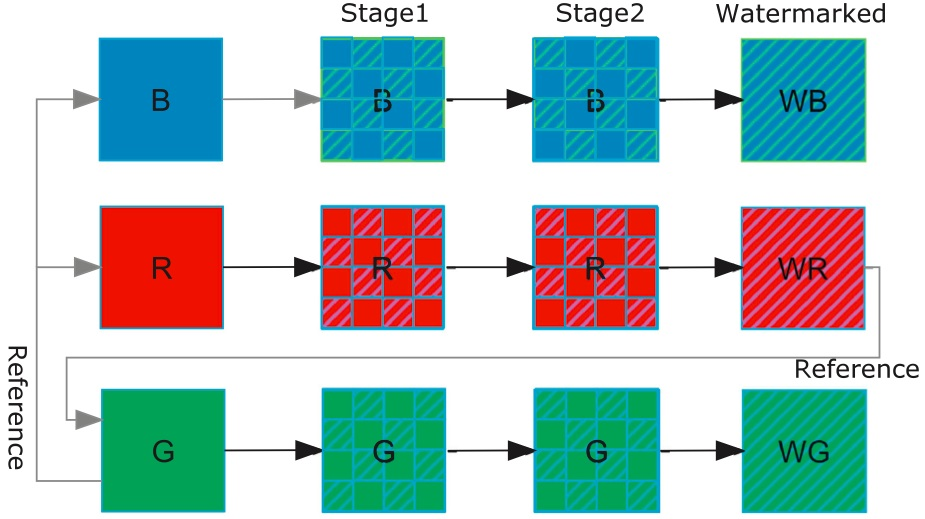
\includegraphics[width=0.65\textwidth]{figures/three_channel_embedding.jpg}
      \caption{彩色图像三个通道嵌入流程图}
      \label{fig:three_channel_embedding}
    \end{figure}
\end{itemize}



\section{实验结果}
\par
在本节,我们将给出所提出的可逆隐藏算法的实验结果。
\begin{figure}[!h]
  \centering 
  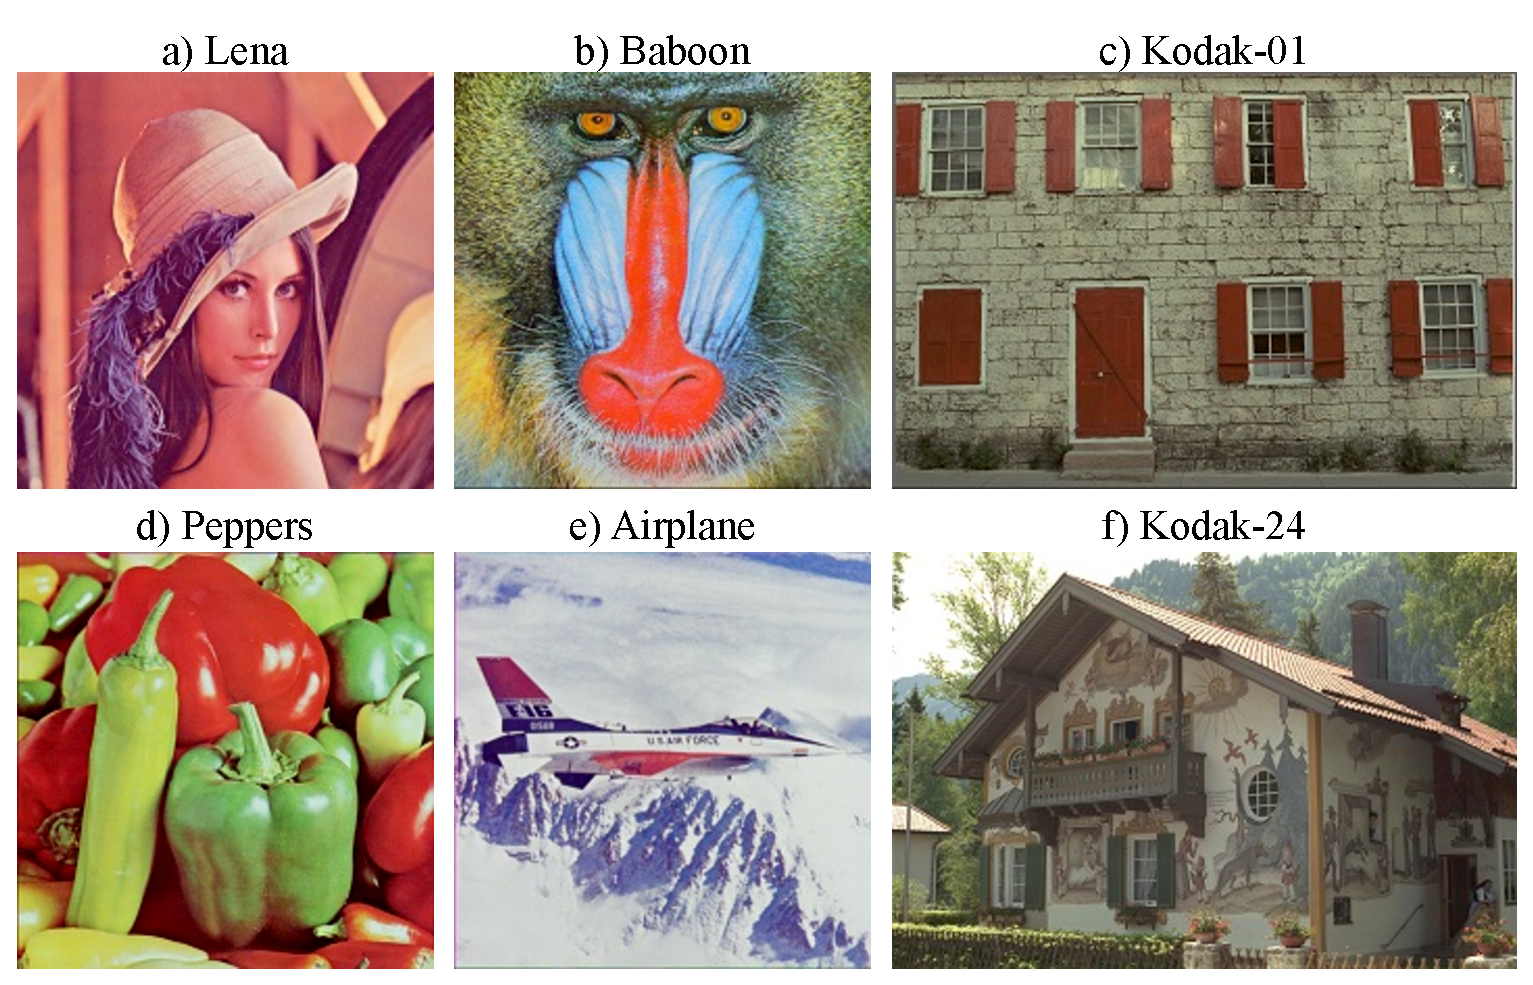
\includegraphics[width=0.9\textwidth]{figures/exp_images.eps}
  \caption{实验用6副彩色图像}
  \label{fig:exp_images}
\end{figure}
\vspace{-7mm}
\par
首先,针对6副彩色图像,我们通过容量-失真曲线研究了提出的算法的性能。容量失真曲
线是一种检验可逆隐藏算法性能的常用手段,以嵌入容量为图像横轴,图像的质量衡量为
纵轴,反映了图像质量同嵌入容量之间的变化关系。在实验中,嵌入容量用嵌入的比特数
表示,图像质量用峰值信噪比(PSNR)来表示。实验用图见图\ref{fig:exp_images},其
中a、b、d、e是$512\times 512$的tiff图像,c、f是两个Kodak图像,大小是$512\times
768$,png格式;6副图像的容量失真曲线如图\ref{fig:6_image_results}。从实验结果
可以看出,本文提出的可逆隐藏算法比文献\cite{li2013reversible}的算法表现更好。
在所有6副图像的结果中,Lena、Baboon、Peppers、Airplane四幅图像的图像质量提升并
不明显,PSNR提升基本都在0.25 dB左右;而Kodak的两幅图像效果提升显著,在2 dB到4 dB
之间。这是由于Kodak两幅图像有较为复杂却规则的纹理,而本文提出的算法能比以往
算法在纹理区域有更好的预测,从而得到更好的实验结果。
\par
随后,我们对UCID数据库超过1300副图像进行了测试,嵌入容量为130000比特,
图\ref{fig:ucid_results}是改进算法图像质量$PSNR_p$同文献\cite{li2013reversible}
算法图像质量$PSNR_{[25]}$的差值直方图。
\begin{figure}[!h]
  \centering 
  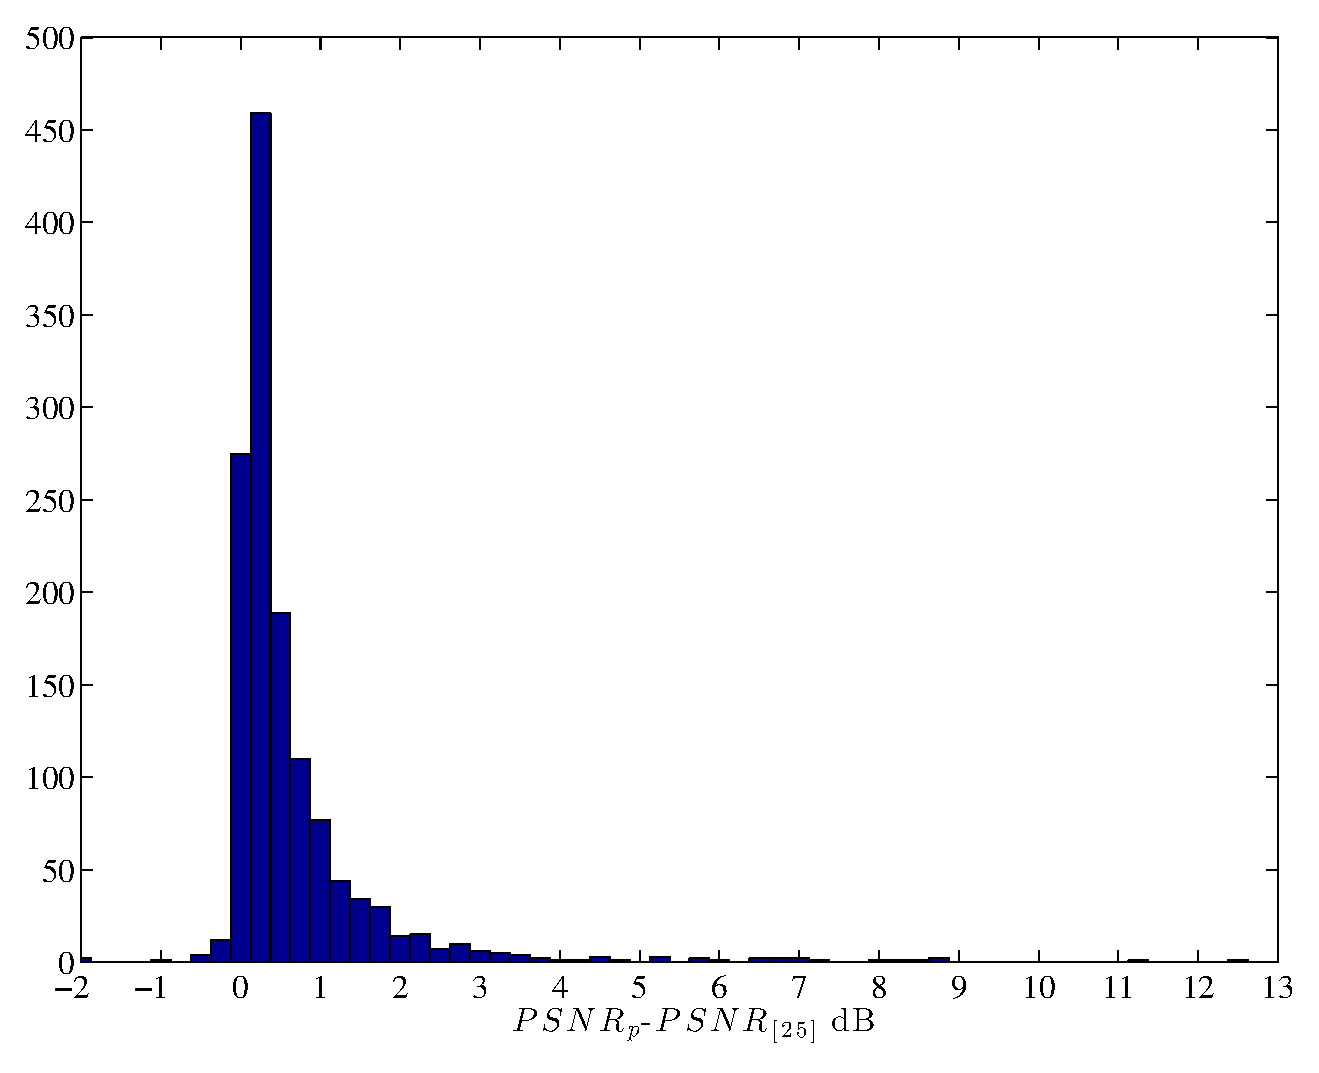
\includegraphics[width=0.9\textwidth]{figures/ucid_results.eps}
  \caption{针对UCID数据库的图像质量提升}
  \label{fig:ucid_results}
\end{figure}
\par
通过图像质量差值我们发现,在超过1000副图像中使用本文提出的算法的图像质量比
使用文献\cite{li2013reversible}的算法图像质量要高,平均PSNR高出0.543 dB,
提升最明显的一幅图像PSNR高出12.474 dB。由此可见,本文提出的算法在绝大多数
情况下都能比文献\cite{li2013reversible}的算法得到更优的结果。
\begin{figure}[!ht]
  \centering 
  \subfigure[Lena]{
    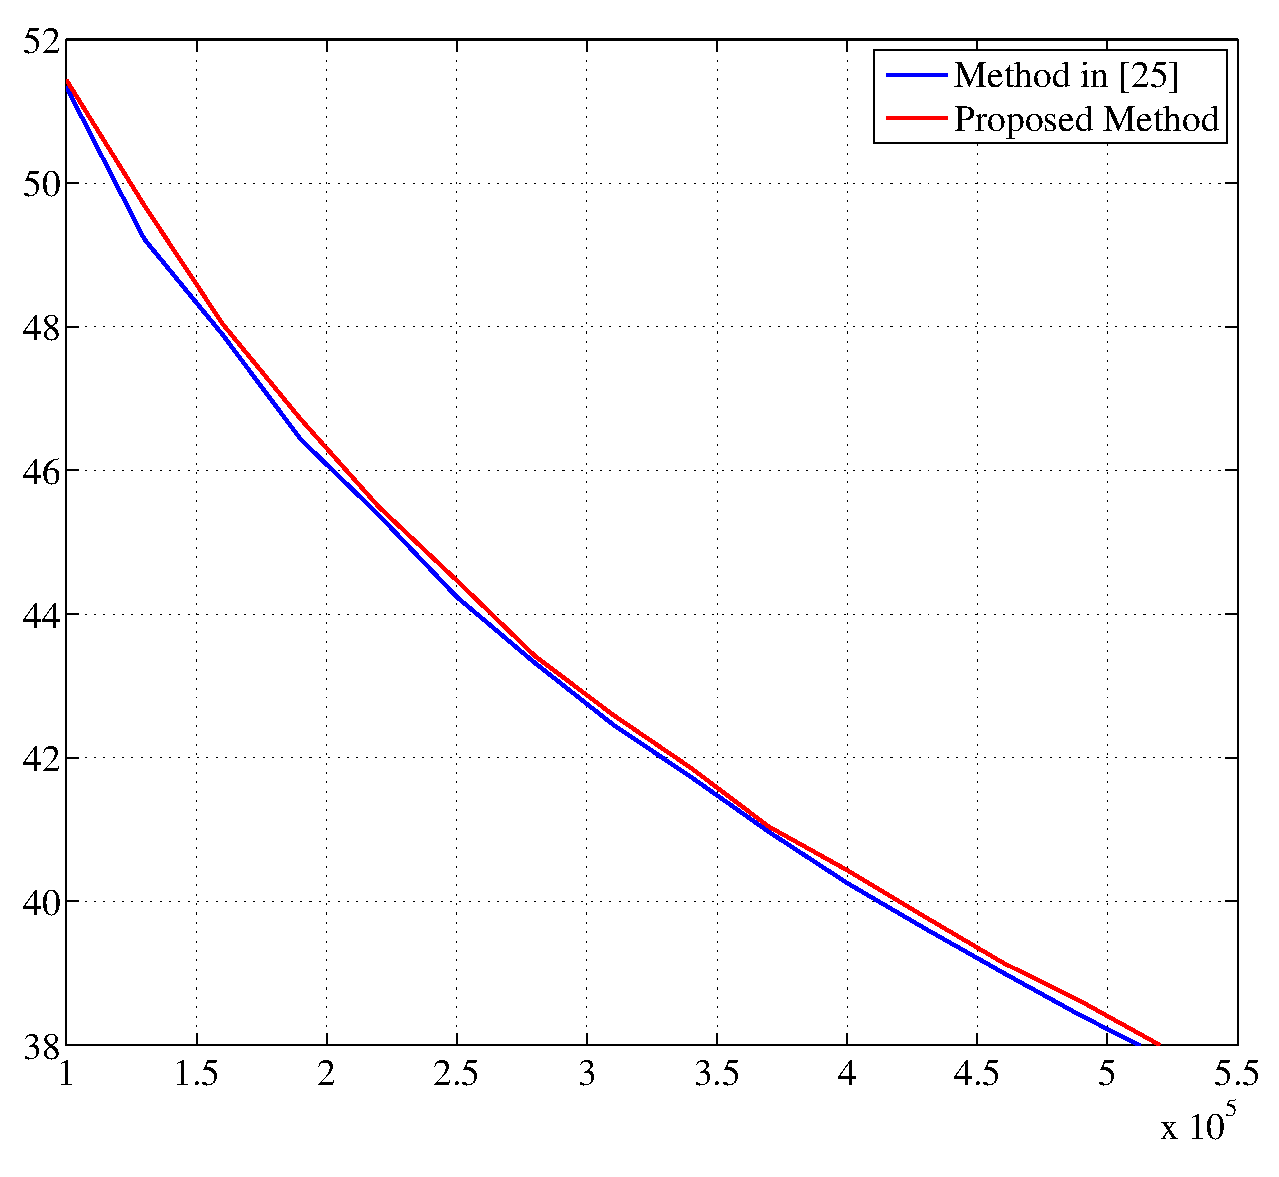
\includegraphics[width=0.4\textwidth]{figures/lena_results.eps}
    \label{fig:lena_results}}
  \subfigure[Baboon]{
    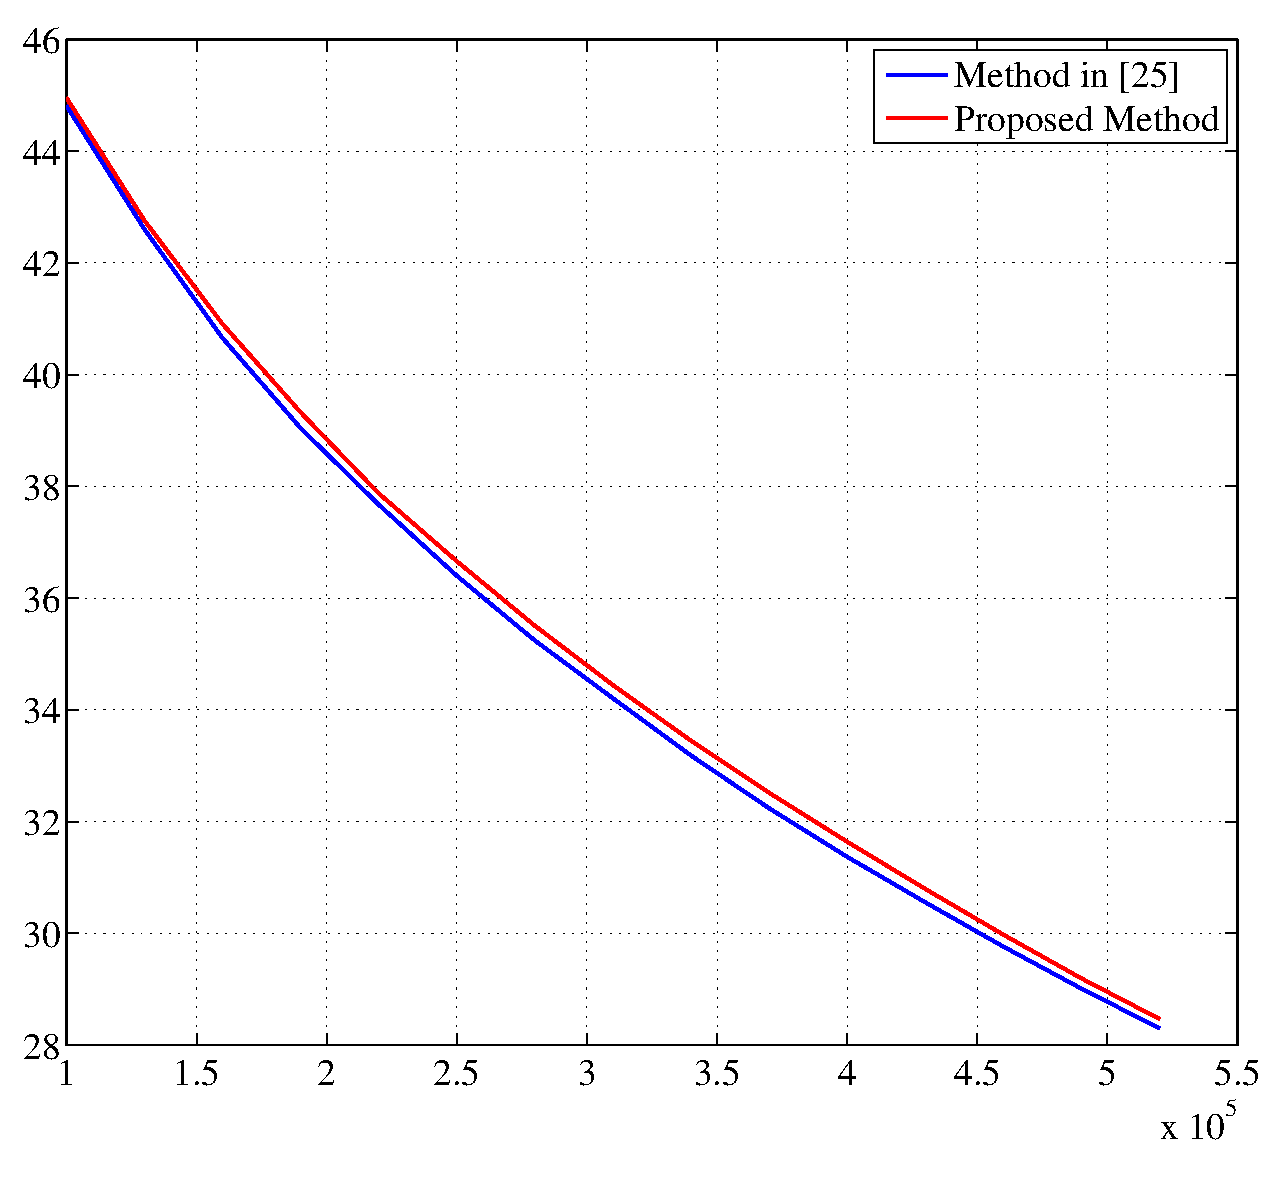
\includegraphics[width=0.4\textwidth]{figures/bab_results.eps}
    \label{fig:lena_results}}\\
  \subfigure[Pepper]{
    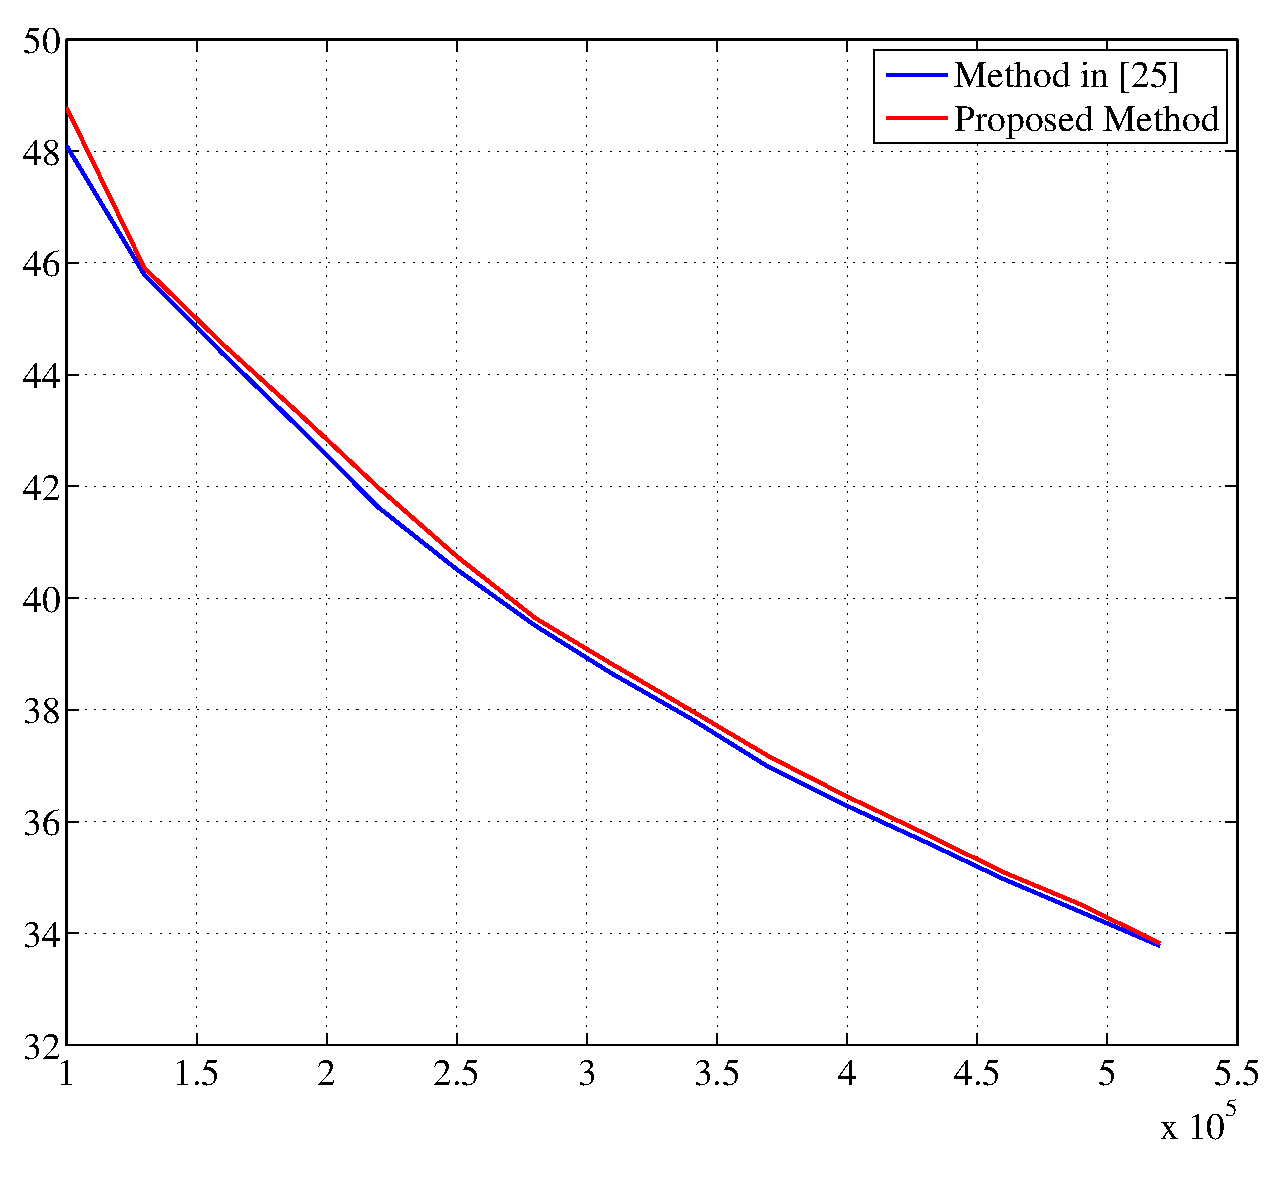
\includegraphics[width=0.4\textwidth]{figures/pep_results.eps}
    \label{fig:lena_results}}
  \subfigure[Airplane]{
    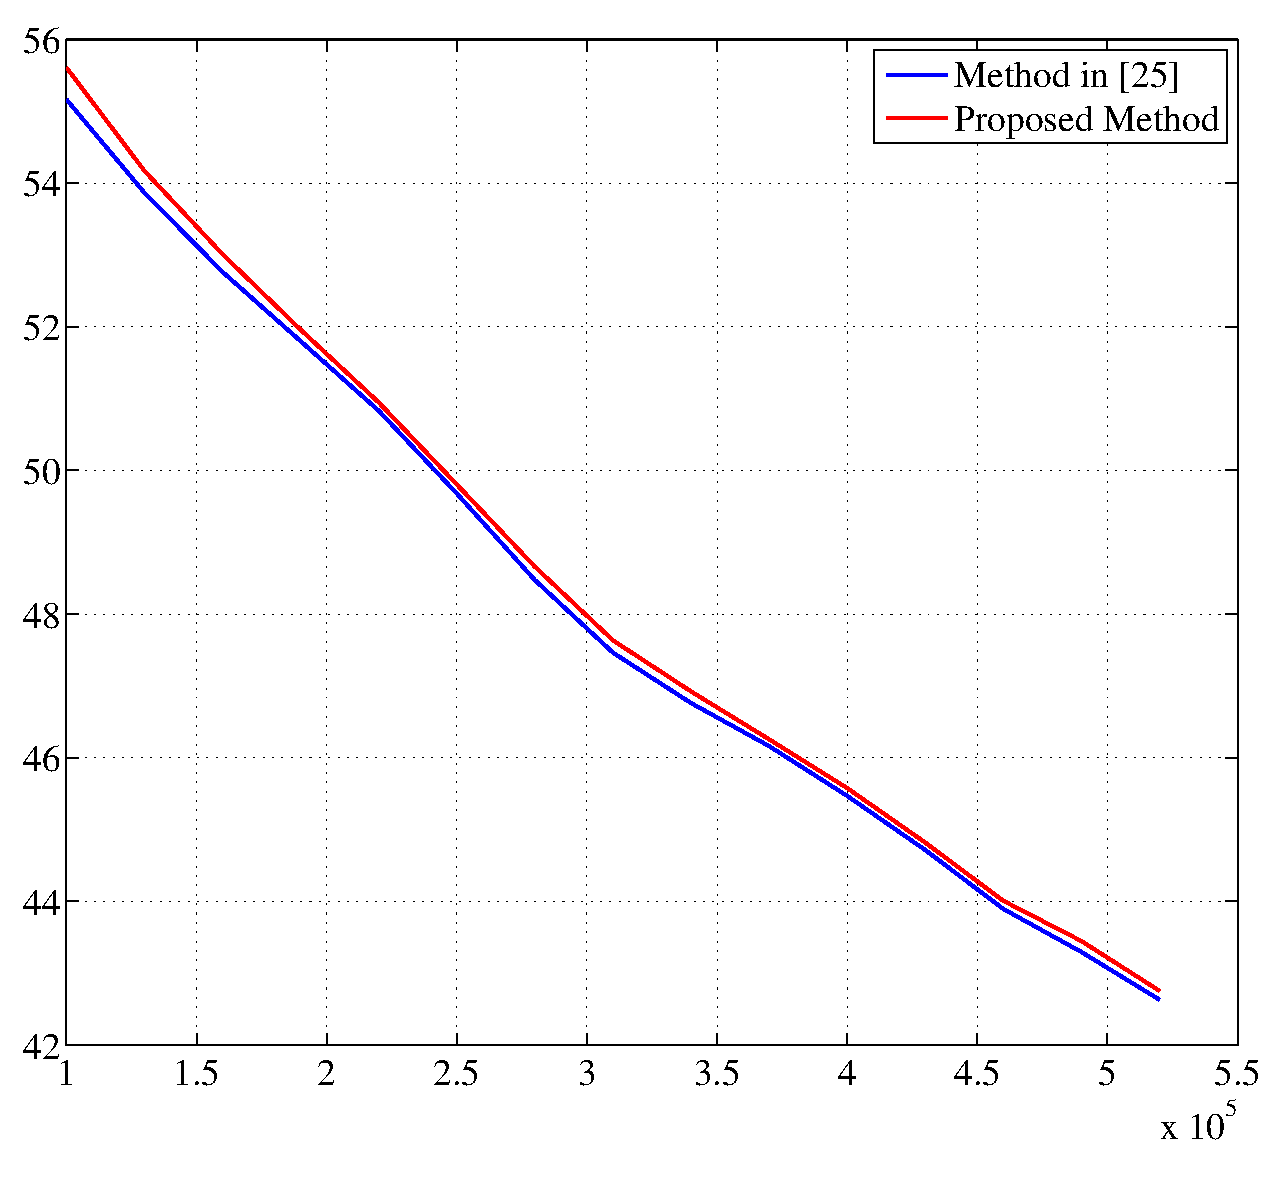
\includegraphics[width=0.4\textwidth]{figures/air_results.eps}
    \label{fig:lena_results}}\\
  \subfigure[Kodak-01]{
    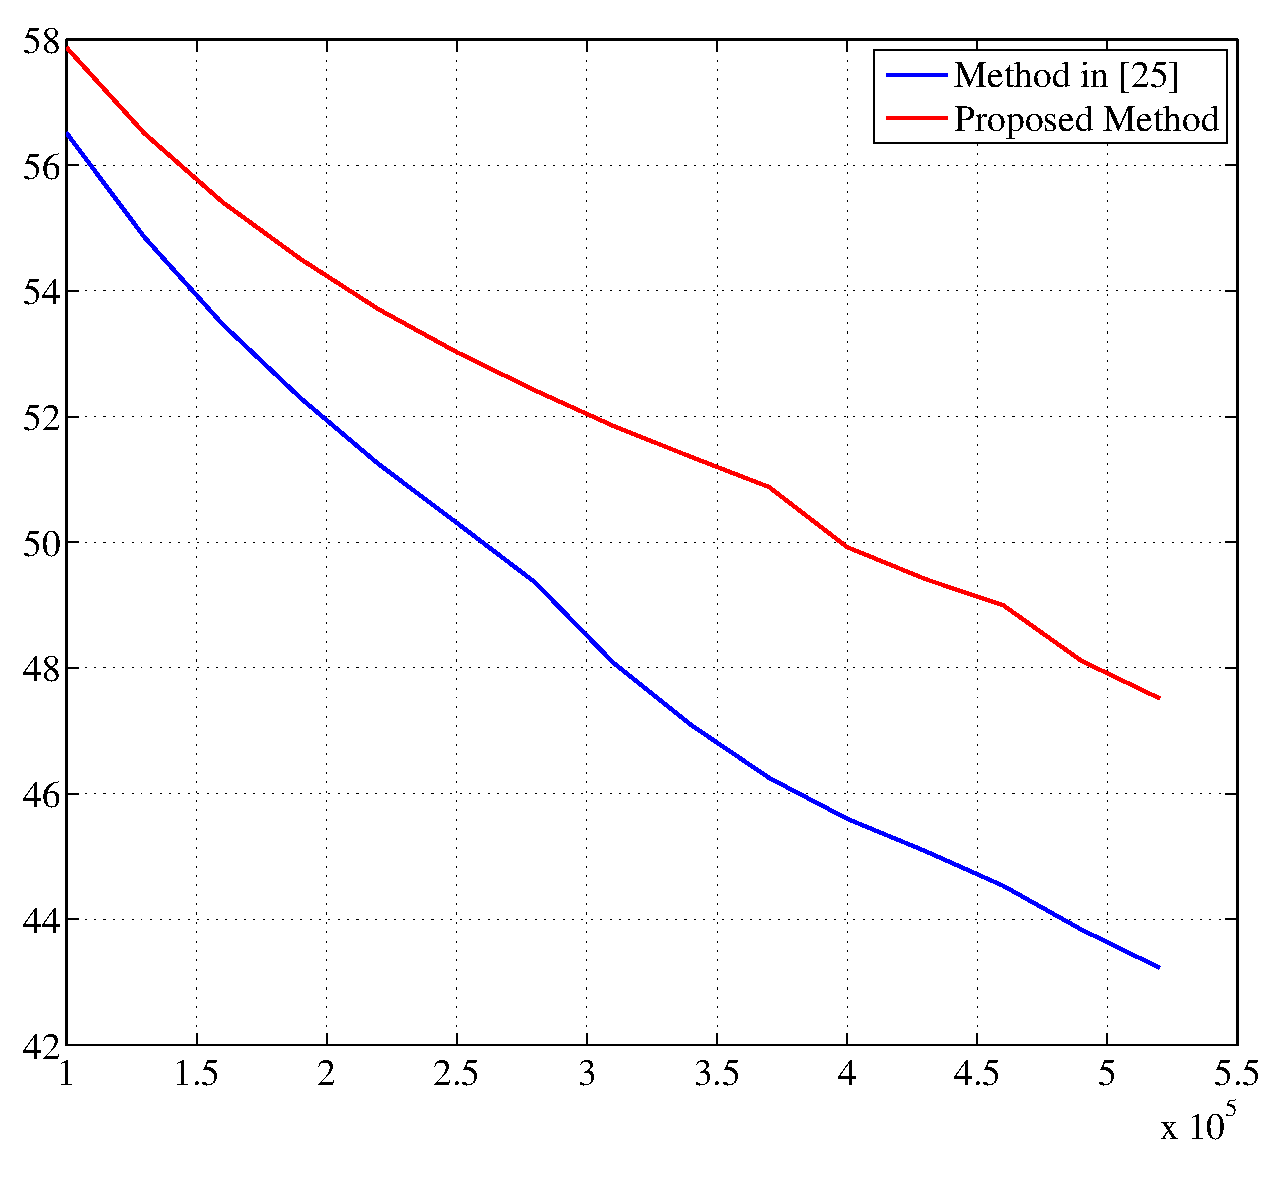
\includegraphics[width=0.4\textwidth]{figures/k1_results.eps}
    \label{fig:lena_results}}
  \subfigure[Kodak-24]{
    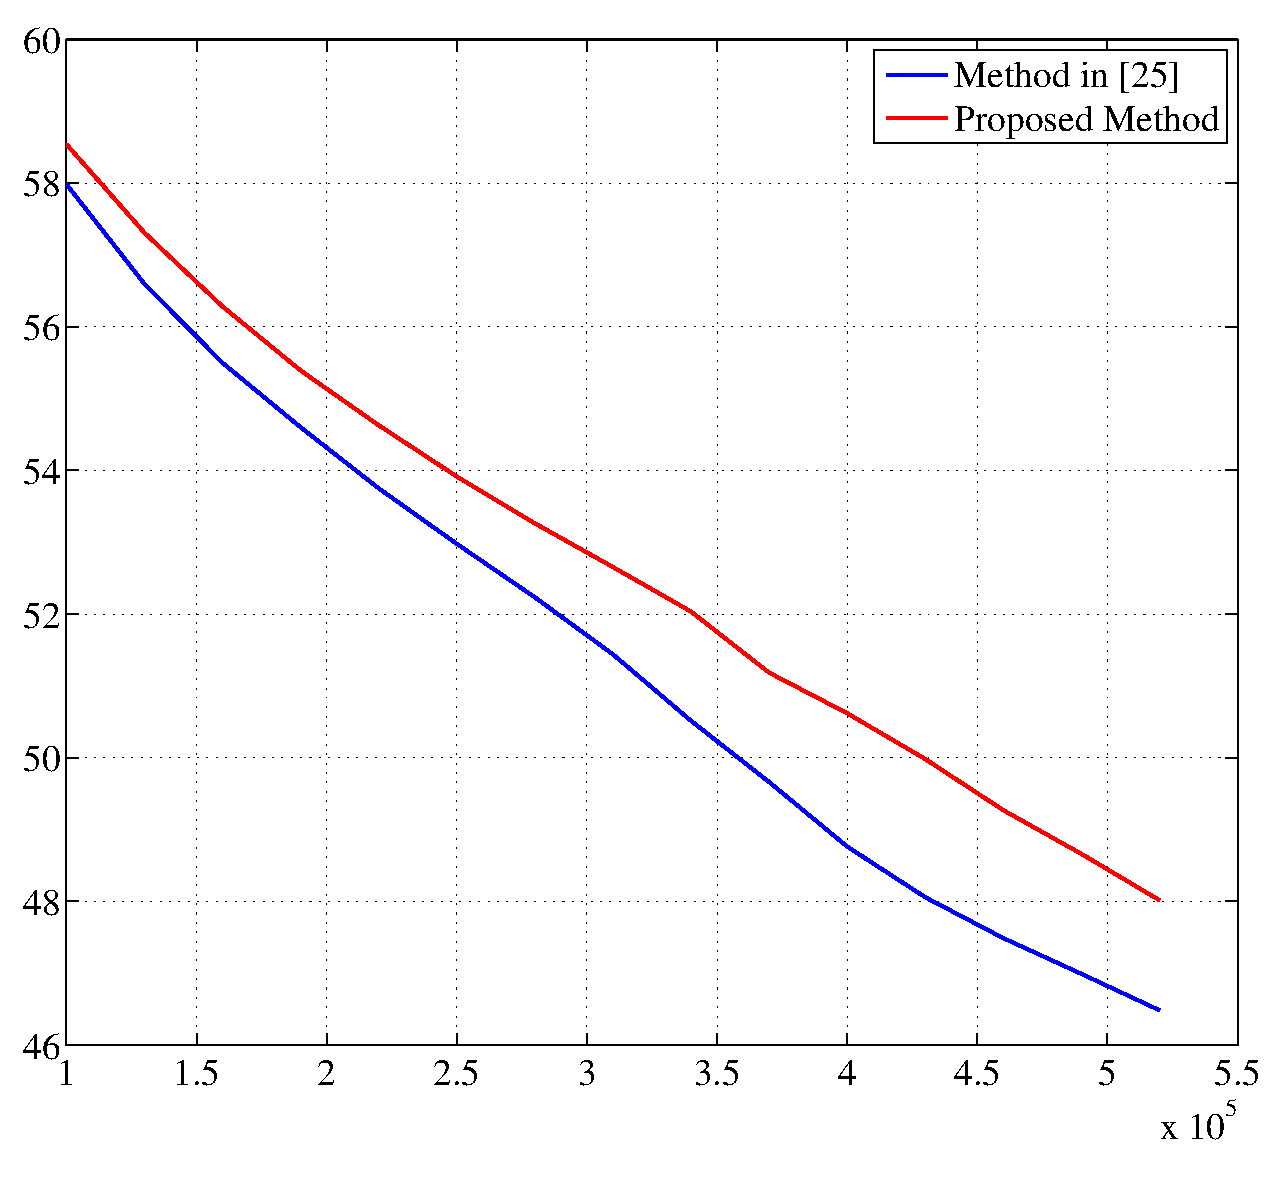
\includegraphics[width=0.4\textwidth]{figures/k2_results.eps}
    \label{fig:lena_results}}\\
  \caption{6副图像的容量失真曲线}
  \label{fig:6_image_results}
\end{figure}
